\documentclass[aspectratio=169]{beamer}
\usepackage{helvet}
\usepackage{calc}
\usepackage[utf8]{inputenc}
\usepackage[english]{babel}

\usetheme{Ilmenau}

\setbeamercovered{transparent}
\setbeamertemplate{navigation symbols}{}

\usepackage{units}
\usepackage{amsbsy}
\usepackage{amsmath}
\usepackage{amssymb}
\usepackage{graphics}
\usepackage{graphicx}
\usepackage{epsf}
\usepackage{epsfig}
\usepackage{fixmath}
%\usepackage{pgfmath}
\usepackage{wrapfig}


\title{Prometheus Deep Dive}
\subtitle{Monitoring. At scale.}
\author{Richard Hartmann \& Frederic Branczyk\\
@TwitchiH \& @fredbrancz}
\date{2018-12-12}


\begin{document}

% hide all subsections
\setcounter{tocdepth}{1}



\section{Introduction}


\subsection{}

\begin{frame}
	\titlepage
\end{frame}


\subsection{}

\begin{frame}
	\frametitle{Who are we?}
	\begin{itemize}
		\item Richard "RichiH" Hartmann
		\begin{itemize}
			\item Swiss army chainsaw at SpaceNet
			\item Project lead for building one of the most modern datacenters in Europe
			\item Debian Developer
			\item FOSDEM, DebConf, DENOGx, PromCon staff
			\item Prometheus team member
		\end{itemize}
		\item Frederic Branczyk
		\begin{itemize}
			\item Red Hat (previously CoreOS)
			\item All things Prometheus / Kubernetes
			\item Kubernetes SIG-Instrumentation lead
			\item Prometheus team member
		\end{itemize}
	\end{itemize}
\end{frame}


\section{Intro}

\subsection{}

% API commitments
% one exporter per service
% focus on services
% failures happen at scale

% HA? run two
% federation
% kein auth/encryption -> reverse proxy


\begin{frame}
	\frametitle{Show of hands}
	\begin{itemize}
		\item Who has heard of Prometheus?
		\item Who is considering to use Prometheus?
		\item Who is POCing Prometheus?
		\item Who uses Prometheus in production?
	\end{itemize}
\end{frame}

\begin{frame}
	\frametitle{Prometheus 101}
	\begin{itemize}
		\item Inspired by Google's Borgmon
		\item Time series database
		\item int64 timestamp, float64 value
		\item Ecosystem of instrumentation \& exporters
		\item Not for events
		\begin{itemize}
			\item Logging
			\item Tracing (more on that later)
			\item etc.
		\end{itemize}
		\item Dashboarding via Grafana
	\end{itemize}
\end{frame}

\begin{frame}
	\frametitle{Main selling points}
	\begin{itemize}
		\item Highly dynamic, built-in service discovery
		\item No hierarchical model, n-dimensional label set
		\item PromQL: for processing, graphing, alerting, and export
		\item Simple operation
		\item Highly efficient
	\end{itemize}
\end{frame}

\begin{frame}
	\frametitle{Cloudy with a chance of buzzwords}
	\begin{itemize}
		\item So it's built with highly dynamic environments in mind
		\item It's the second project to ever join CNCF and the de facto standard in cloud-native monitoring
		\item Kubelets, sidecars, microservices, ALL the cloud-native
		\vfill
		\item But it's a monolithic application
		\vfill
		\item ...why?
	\end{itemize}
\end{frame}

\begin{frame}
	\frametitle{Resilience, resilience, and also resilience}
	\begin{itemize}
		\item What do you need for operations?
		\begin{itemize}
			\item Power and cooling
			\item Network connectivity
			\item Observability, a.k.a. Monitoring
		\end{itemize}
		\item The rest you can fix
	\end{itemize}
\end{frame}


%%TODO What was stable release
\section{2.0 to 2.2.1}
\subsection{}

\begin{frame}
	\frametitle{Three main features}
	\begin{itemize}
		\item Storage backend
		\begin{itemize}
			\item Caveat: Prometheus 2.0 comes with storage v3
		\end{itemize}
		\item Staleness handling
		\item Remote read \& write API is now stable-ish
		\item Links to in-depth talks about these features are at the end
	\end{itemize}
\end{frame}


\subsection{Storage}

\begin{frame}
	\frametitle{Prometheus 1.x}
	\begin{itemize}
		\item We used to have one file per time series
		\item ..and one common index for all of time
		\item Relatively easy to implement
		\item Pretty efficient
		\item Why change?
	\end{itemize}
\end{frame}

\begin{frame}
	\frametitle{Churn}
	\begin{itemize}
		\item Churn was becoming more and more of a problem
		\item There's a company with a 15 minute maximum lifetime for their containers
		\item If you have a lot of files which might contain data for any given time frame, you need to look at all of them
	\end{itemize}
\end{frame}

%\begin{frame}
%	\frametitle{Storage v3}
%	\begin{itemize}
%		\item Fabian Reinartz had an idea about new storage
%		\item This POC turned out to be so good, we decided to cut a major release for it
%		\item How does it work?
%	\end{itemize}
%\end{frame}

\begin{frame}
	\frametitle{One file per series}
	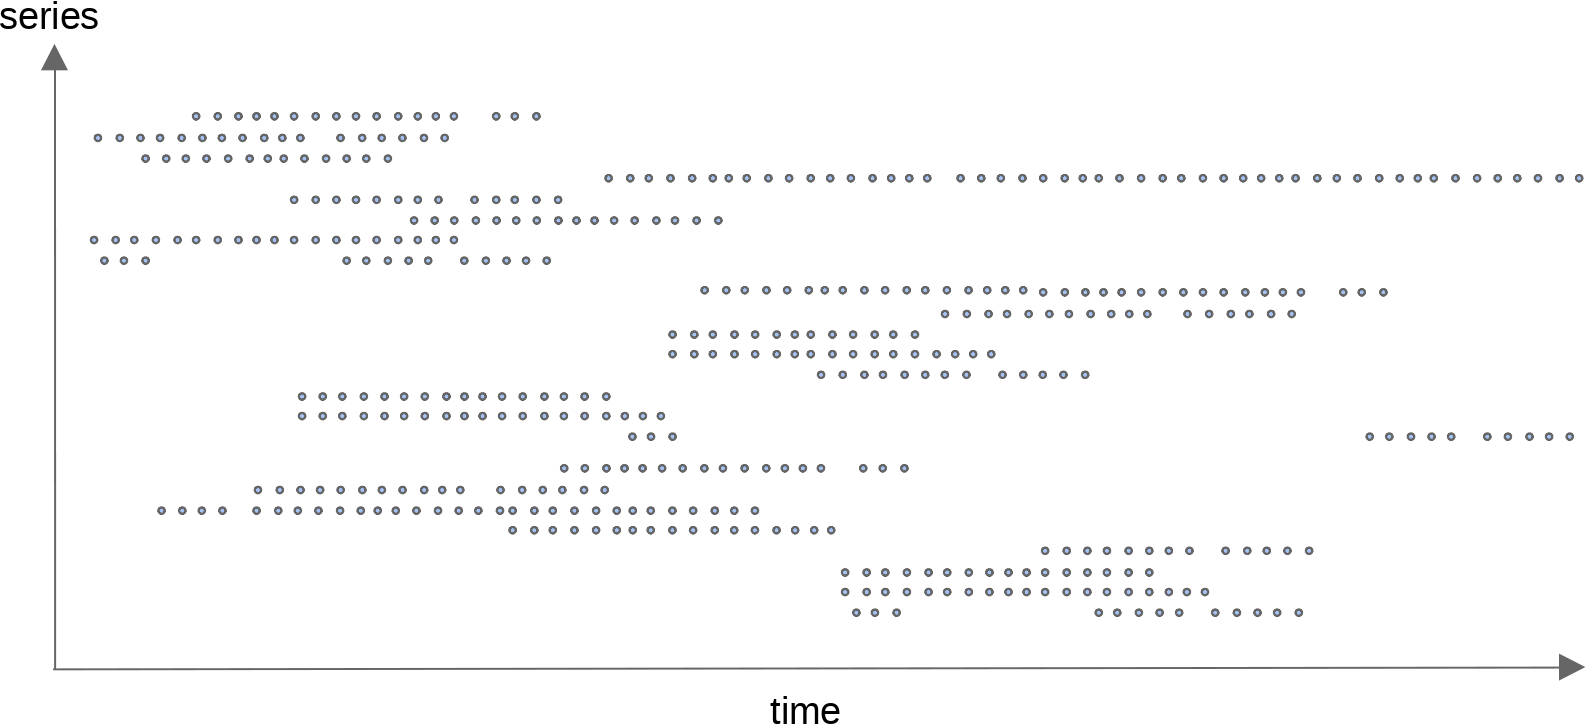
\includegraphics[width=\textwidth]{storage--file_per_series.png}
\end{frame}

\begin{frame}
	\frametitle{Selection}
	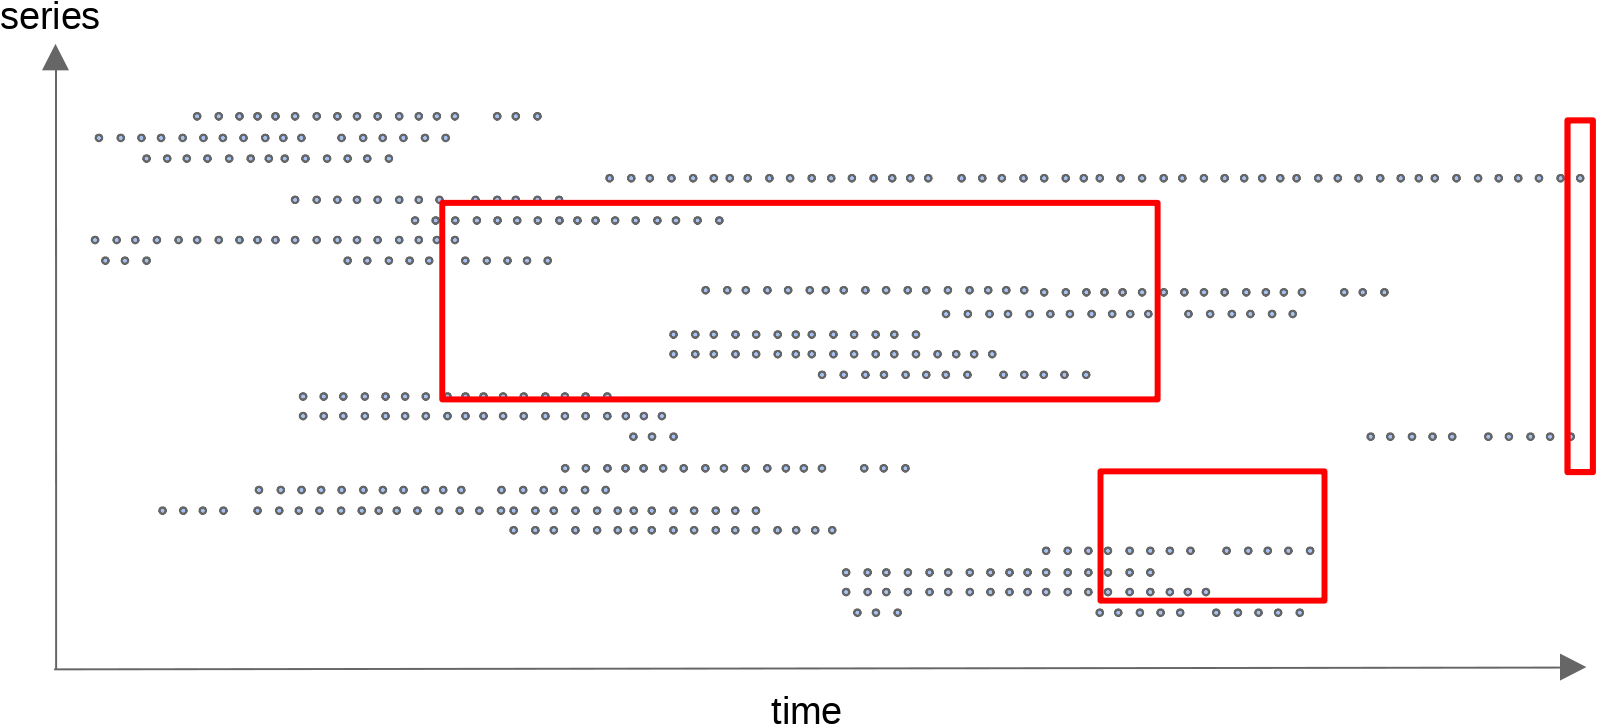
\includegraphics[width=\textwidth]{storage--file_per_series_with_selection.png}
\end{frame}

\begin{frame}
	\frametitle{Blocks}
	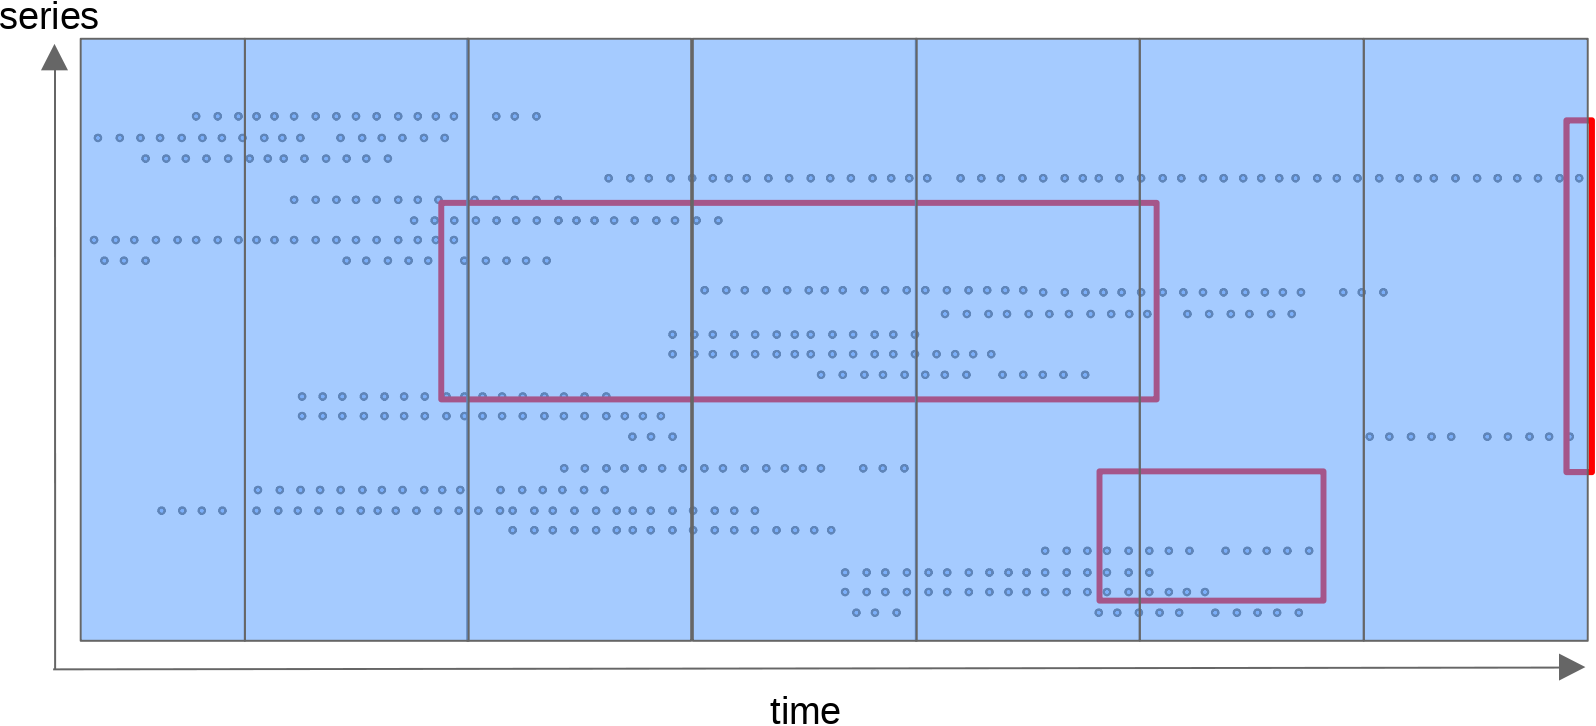
\includegraphics[width=\textwidth]{storage--block_with_selection.png}
\end{frame}

%\begin{frame}
%	\frametitle{Storage v3}
%	\begin{itemize}
%		\item Deletions set tombstones
%		\item Actual deletion done via compaction runs, or triggered by large tombstone ratio
%		\item Oh, and we now simply mmap storage blocks into RAM and let the OS handle the rest
%	\end{itemize}
%\end{frame}

\begin{frame}
	\frametitle{Test setup}
	\begin{itemize}
		\item Kubernetes cluster with dedicated Prometheus nodes
		\item 800 microservice instances and Kubernetes components
		\item 120k samples/sec
		\item 300k active time series
		\item Swap out 50\% of all pods every 10 minutes
	\end{itemize}
\end{frame}

\begin{frame}
	\frametitle{Results}
	\begin{itemize}
		\item 15x reduction in memory usage
		\item 6x reduction in CPU usage
		\item 80-100x reduction in disk writes
		\item 5x reduction in on-disk size
		\item 4x reduction in query latency on expensive queries
		\item Want to reproduce? \url{https://github.com/prometheus/prombench}
	\end{itemize}
\end{frame}

%%%%%%%%%%%%%%%%%%%\begin{frame}
%%%%%%%%%%%%%%%%%%%	\frametitle{Other 2.x news}
%%%%%%%%%%%%%%%%%%%	\begin{itemize}
%%%%%%%%%%%%%%%%%%%		\item Snapshotting and backing up Prometheus works
%%%%%%%%%%%%%%%%%%%		\item New staleness handling
%%%%%%%%%%%%%%%%%%%	\end{itemize}
%%%%%%%%%%%%%%%%%%%\end{frame}



\subsection{Remote read API}

\begin{frame}
	\frametitle{Playing nicely with others}
	\begin{itemize}
		\item We now have a stable-ish remote read/write API
		\item Twelve integrations for this API
		\item Ongoing work to send write-ahead-log over the wire to fill gaps
	\end{itemize}
\end{frame}


\subsection{Stability}

\begin{frame}
	\frametitle{Security \& quality}
	\begin{itemize}
		\item CNCF sponsored external code review by Cure53
		\item Focussed on security, but this always means looking at stability as well
		\item Keep in mind that Prometheus willfully ignored most security considerations
		\item Encryption, authentication, and authorization currently need to be handled via reverse proxies
		\item We will be changing Prometheus to support security out-of-the-box
	\end{itemize}
\end{frame}

\begin{frame}
	\frametitle{Release stability}
	\begin{itemize}
		\item Every single release since 2.0.0 has had issues
		\item Some bugs and some human mistakes in the release process
		\item Always running latest is the cloud-native approach, but this is still not acceptable
		\item ..especially if every single version has its issues
		\item We put in more checks and balances to ensure cleaner releases going forward
		\item If there are bugs we can't get rid of, we go into feature moratorium
		\item 2.3.2 is the first fully stable release in the 2.x train
	\end{itemize}
\end{frame}


\section{2.4 - 2.6}


\subsection{Release cycle}

\begin{frame}
	\frametitle{Fixed release cycle}
	\begin{itemize}
		\item Every six weeks, we mark a new RC
		\item Cycle is relative to previous RC, not previous release
		\item RC is published and iterated upon as long as there are issues
		\item Release handling cycles between team members to ensure several people are able to release
	\end{itemize}
\end{frame}


\subsection{PromQL}

\begin{frame}
	\frametitle{Quick is not quick enough}
	\begin{itemize}
		\item Brian Brazil optimized PromQL
		\item 5x faster for time vector functions
		\item 100x reduction in garbage to collect
	\end{itemize}
\end{frame}


\subsection{Long-term storage}

\begin{frame}
	\frametitle{Problem statement}
	\begin{itemize}
		\item Long-term storage is one of the last remaining major features left untackled
		\item Fundamentally, Prometheus operates as distinct data islands
		\item As there's no backfill, data dies along with its instance by default
	\end{itemize}
\end{frame}

\begin{frame}
	\frametitle{Solutions}
	\begin{itemize}
		\item Storage v3 supports backups efficiently and effectively
		\item Remote read-write allows you to integrate with a growing list of projects and products, e.g. Cortex
		\item On storage level, there are object storage backends for Prometheus, e.g. Thanos
		\item Remote API can now send WAL over the wire to fill gaps in data
		\item There are twelve different systems which are able to ingest Proemtheus data this way
		\item We deliberately do no endorse any particular approach or solution; this might change over time
	\end{itemize}
\end{frame}

\begin{frame}
	\frametitle{Testing}
	\begin{itemize}
		\item Unit tests for alerts
		\item Our goal is to allow end-to-end testing of not only Prometheus as software, but also of any individual deployment
	\end{itemize}
\end{frame}

\section{Beyond}

\subsection{ACID}

\begin{frame}
	\frametitle{ACID databases...}
	\begin{itemize}
		\item \textbf{A}tomicity - since 1.x
		\item \textbf{C}onsistency - since 1.x
		\item \textbf{I}solation - will happen within 2.x
		\item \textbf{D}urability - since 2.0
	\end{itemize}
\end{frame}

\begin{frame}
	\frametitle{Isolation}
	\begin{itemize}
		\item Each append action gets a write ID (64 bit monotonic counter)
		\item Every sample's write ID is noted along with value and timestamp
		\item Any append action which has not yet been committed, or has been rolled back, is ignored at query time
		\item We keep write IDs in memory; if we restart or crash, the atomicity of the write ahead log will protect us
	\end{itemize}
\end{frame}

\subsection{OpenMetrics}

\begin{frame}
	\frametitle{Humble aspirations}
	\begin{itemize}
		\item When we say that we want to change how the world does monitoring, we mean it
		\item One of our most powerful features are labels
		\item Labels are encoded in our exposition format
		\item Some third-party projects and vendors have an issue with supporting a "competing" project
	\end{itemize}
\end{frame}

\begin{frame}
	\frametitle{What do?}
	\begin{itemize}
		\item We are spinning out Prometheus' exposition format
		\item Face-to-face kick-off last August at Google London
		\item Independent CNCF member project, IETF RFC, test suite, etc
		\item We are writing code in Prometheus and the Python client library
		\item \url{https://github.com/OpenObservability/OpenMetrics}
		\item Prometheus 2.5 has experimental OpenMetrics support
	\end{itemize}
\end{frame}

\begin{frame}
	\frametitle{Beyond metrics}
	\begin{itemize}
		\item OpenMetrics supports more than just metrics
		\item Every single data point in a time series can point to one single event
		\item Especially useful if you emit one trace id per histogram bucket
		\item Some integrations already support this concept, e.g. OpenCensus
		\item Ingestors are free to discard this optional data, e.g. Prometheus
	\end{itemize}
\end{frame}

\begin{frame}
	\frametitle{Bringing observability together}
	\begin{itemize}
		\item OpenTracing already on board with this effort
		\item There will be an observability sidetrack
		\item Long-term goal is one common, modular, well-engineered standard under a new name
	\end{itemize}
\end{frame}



\begin{frame}
	\frametitle{First committers to adopt, too many to list all}
	\begin{itemize}
		\item Cloudflare
		\item CNCF at large
		\item GitLab
		\item Google
		\item Grafana
		\item InfluxData
		\item Kausal.co
		\item Oath.com / Yahoo / Verizon
		\item RobustPerception
		\item SpaceNet
		\item Uber
	\end{itemize}
\end{frame}


\subsection{Long term promises}

\begin{frame}
	\frametitle{Generally speaking...}
	\begin{itemize}
		\item Yes, we want to change the world
		\item Simple and resilient operation of Prometheus remains a core goal
		\item The path from raw data to reliable alerts is the single most important user contract we have
		\item More project and software integrations... and we're talking to hardware vendors as well
		\item Supporting tomorrow's 10x scale today
	\end{itemize}
\end{frame}



\section{Outro}


\subsection{}

\begin{frame}
	\frametitle{Relevant talks}
	\begin{itemize}
		\item Storing 16 Bytes at Scale: \url{https://promcon.io/2017-munich/talks/staleness-in-prometheus-2-0/}
		\item Staleness and Isolation in Prometheus 2.0: \url{https://promcon.io/2017-munich/talks/staleness-in-prometheus-2-0/}
		\item Social aspects of change: \url{https://promcon.io/2017-munich/talks/social-aspects-of-change/}
	\end{itemize}
\end{frame}


\begin{frame}
	\frametitle{Further reading}
	\begin{itemize}
		\item Prometheus 2017 Dev Summit: \url{https://docs.google.com/document/d/1DaHFao0saZ3MDt9yuuxLaCQg8WGadO8s44i3cxSARcM/edit}
		\item Prometheus 2018 Dev Summit: \url{https://docs.google.com/document/d/1-C5PycocOZEVIPrmM1hn8fBelShqtqiAmFptoG4yK70/edit}
		\item OpenMetrics: \url{https://github.com/RichiH/OpenMetrics}
		\item This and other talks: \url{https://github.com/RichiH/talks/}
	\end{itemize}
\end{frame}

\begin{frame}
	\frametitle{Thanks!}
		\begin{center}
			\vfill
			Thanks for listening!\\
			\vfill
			Questions?
			\vfill
%			See slide footer for contact info.
%			\vfill
		\end{center}
\end{frame}

\end{document}

%\begin{frame}
%	\frametitle{}
%	\begin{itemize}
%		\item 
%		\item 
%		\item 
%		\item 
%		\item 
%	\end{itemize}
%\end{frame}
